\chapter{Fluxograma} \label{fluxograma}
\par Atualmente a disseminação do conceito lógico computacional estruturado textual, que envolve raciocínio lógico ou de sintaxe pesada, possui uma didática, utilizada empiricamente por professores da área, que tornam difícil o aprendizado do aluno. [Rocha 1991] e [Chen e Morris 2005]
\par Sabe-se que o ser humano possui mais habilidade em interpretar algoritmos em forma visual do que em formato texto. Isto se deve ao fato que o hemisfério esquerdo do cérebro processar informação oral e lógica, enquanto o hemisfério direito processa informação visual e espacial. Quando interpretarmos um texto o hemisfério direito não contribui de forma significativa para o aprendizado. [Da Silva 2001]
\par Assim a utilização de fluxogramas e outras formas de interpretação visual, de algoritmos lógicos computacionais textualmente estruturados, torna mais fácil o aprendizado, pois estimula ambos os lados do cérebro.
\par Neste sentido, este projeto tem como proposta, identificar e expor na forma de fluxogramas, a analise de algoritmos determinísticos não recursivos, escritos na linguagem C.

\begin{figure}[htp!]
\centering
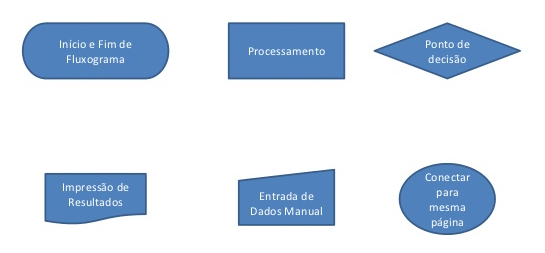
\includegraphics[width=\textwidth]{figuras/fluxograma2.png}
\caption{Formatos para geração de fluxograma}
\label{figura1}
\end{figure}

\begin{figure}[htp!]
\centering
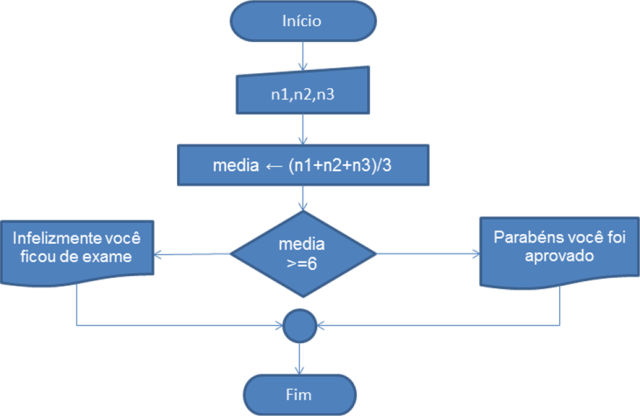
\includegraphics[width=\textwidth]{figuras/fluxograma1.jpg}
\caption{Exemplo de fluxograma final}
\label{figura2}
\end{figure}
% \chapter{ESTUDO DE VIABILIDADE} \label{estudo}

% Neste capítulo pretende-se mostrar por que o \textit{software} proposto será viável para áreas comerciais de qualquer ramo. As próximas seções falam sobre o mercado potencial, os benefícios, as oportunidades, as forças, as fraquezas, as ameaças e os concorrentes diferenciais.

% \section{Mercado potencial}

% \section{Benefícios}

% \section{Oportunidades}

% \section{Forças}

% \section{Fraquezas}


% \section{Ameaças}


% \section{Concorrentes Diferenciais}

